\section{Evaluation and Experiments}
We have evaluated the performance of the event driven workflow tool on Caliburan cluster at Rutgers Discovery Informatics Institute. The Caliburan cluster is based on a FatTwin SuperServer system. It has 560 nodes, each with two Intel Xeon E5-2695 v4 (Broadwell) processors, 256 gigabytes (GB) of RAM, and a 400 GB Intel NVMe drive. Overall, the system has 20,160 cores, 140 TB of memory and 218 TB of non-volatile memory. The performance is 603 TFLOPS with a peak performance of 677 TFLOPS\cite{caliburn}.

\subsection{Performance Evaluation}
The first experiment is measure the latency of task triggering time. The test using synthetic workflow include two tasks, taskB depends on taskA. Our test based on the workflow pattern in Figure 2 which include aggregation, broad caster and chained pattern. For every latency, we also compare our workflow tool with the other workflow tool Swift\cite{wilde2011swift} and Makeflow\cite{albrecht2012makeflow}.

For chained pattern when taskA.X finish taskB.X will be triggered, we increase the number of coupling pairs of (taskA.X, taskB.X) to test the latency.

For aggregation pattern, there are several taskA.X and one taskB, when all taskA.X finished, task.B will be triggered and we will test waiting time of the taskB with the increasing number of taskA.X

For broadcaster pattern, there are one taskB and several taskA.X, when taskA finish, all the task.B will be triggered and we will test the average waiting time of the taskB with the increasing of the taskB.X.

\subsection{hybrid workflow using scenarios}
In this part, we use a real use case to show how event workflow tool compose different abstraction of task and leverage the scientific application.
Figure ? shows the different between the traditional post-processing workflow and the hybrid event driven workflow. We could notice that in-situ task and the post-processing task could be composed together by event driven workflow and the synchronization between different task is also minimized by event messages.

\begin{figure} 
\centering
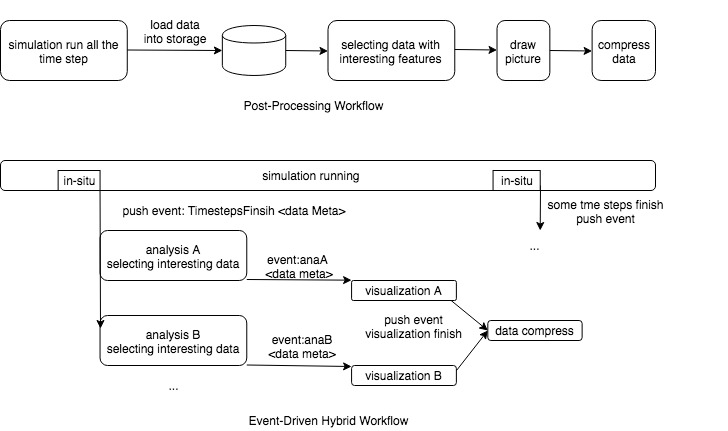
\includegraphics[width=1.0\linewidth]{./figure/hybridapplication.jpg}
\caption{Scientific Workflow Pattern}
 \label{fg:state}
\end{figure} 